\section{Xây dựng bài toán}
\label{sec:problem-formulation}

Mục tiêu điều khiển là đưa quadcopter lần lượt đi qua chuỗi waypoint
\(\mathcal{W} = \{\mathbf{w}_1, \ldots, \mathbf{w}_N\}\), như minh họa trong Hình~\ref{fig:problem-formulation}, trong không gian ba chiều. Waypoint thứ \(i\),
\(\mathbf{w}_i = [x_i, y_i, z_i]^{\mathsf{T}}\), và vị trí của quadcopter tại thời điểm \(t\),
\(\mathbf{p}_t = [x_t, y_t, z_t]^{\mathsf{T}}\), đều được biểu diễn trong hệ tọa độ quán tính North--East--Down (NED).
\begin{figure}[H]
    \centering
    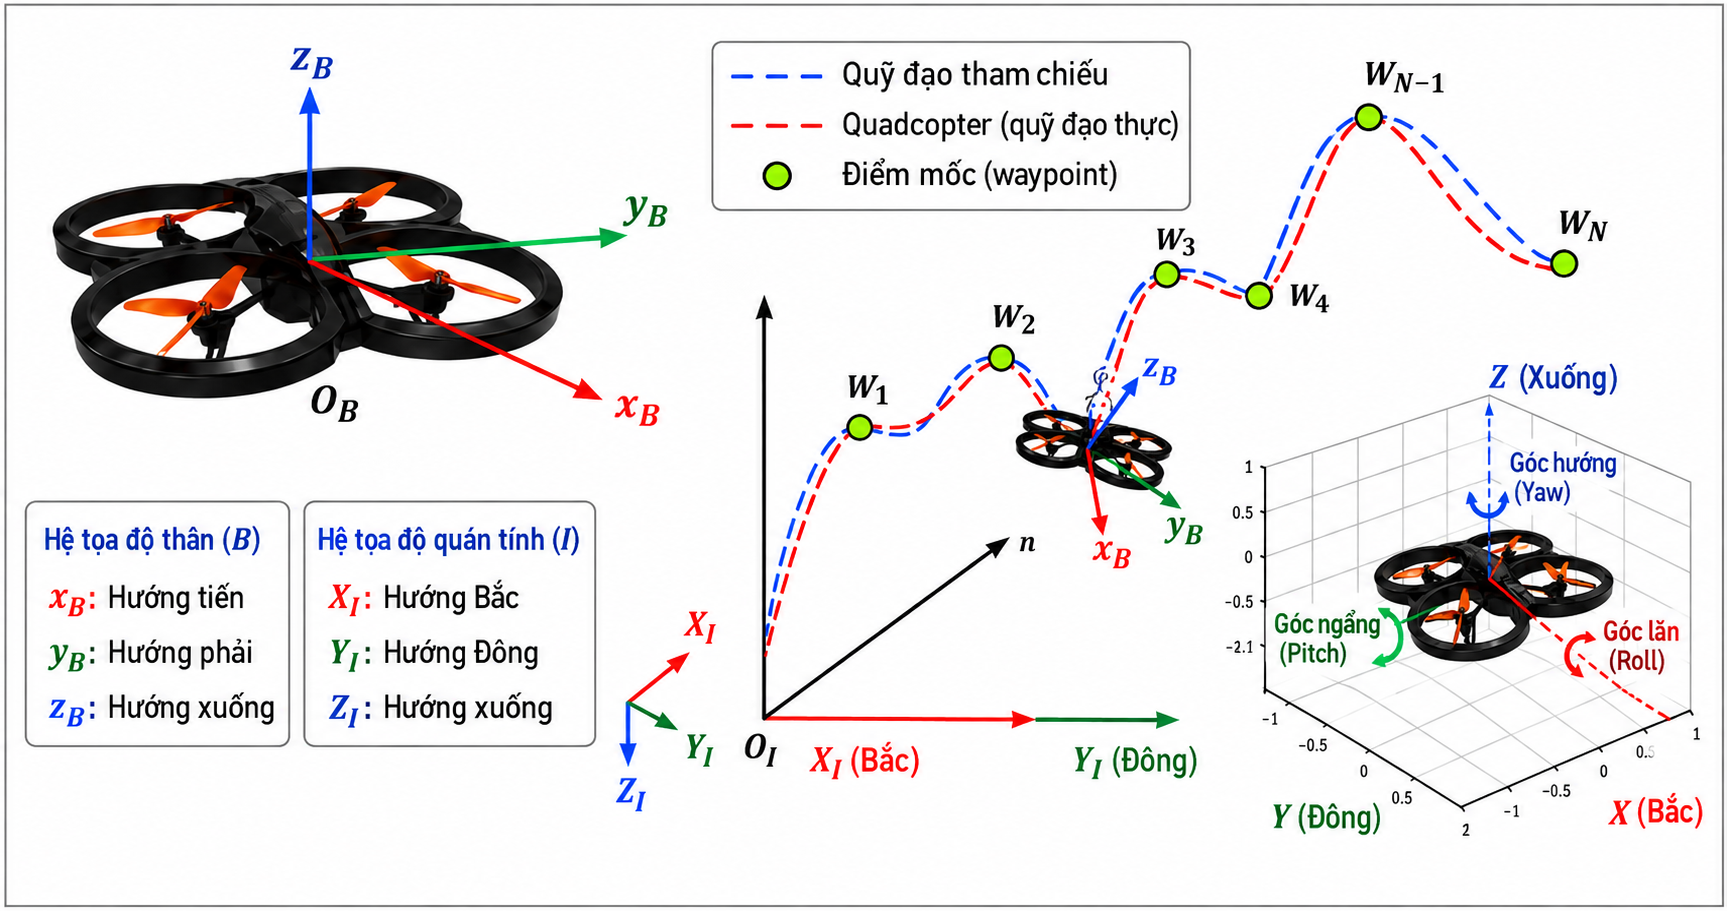
\includegraphics[width=\columnwidth]{Figure/image.png}
    \caption{Mô hình bài toán bám quỹ đạo waypoint của quadcopter.}
    \label{fig:problem-formulation}
\end{figure}
Trong Hình~\ref{fig:problem-formulation}, chuyển động của quadcopter được mô tả thông qua hai hệ tọa độ: hệ tọa độ quán 
tính \(\{I\}\) và hệ tọa độ thân \(\{B\}\). Hệ tọa độ quán tính được sử dụng để mô tả vị trí và quỹ đạo bay của quadcopter 
trong không gian toàn cục, với các trục \(X_I\), \(Y_I\), và \(Z_I\) lần lượt tương ứng với các hướng North, East, và Down. 
Trong khi đó, hệ tọa độ thân gắn trực tiếp với quadcopter gồm các trục \(x_B\), \(y_B\), và \(z_B\), dùng để mô tả hướng 
chuyển động và tư thế của phương tiện. 